\documentclass[twocolumn]{article}

%% Language and font encodings
\usepackage[english]{babel}
\usepackage[utf8]{inputenc}
\usepackage{csquotes}
\bibliographystyle{unsrt}
\usepackage{booktabs}

\usepackage{tabu}
\usepackage[T1]{fontenc}

%% Sets page size and margins
\usepackage[a4paper,top=2cm,bottom=2cm,left=3cm,right=3cm,marginparwidth=1.75cm]{geometry}

%% Useful packages
\usepackage{amsmath}
\usepackage{graphicx}
%\usepackage{apacite}
\usepackage[colorinlistoftodos]{todonotes}
\usepackage[colorlinks=true, allcolors=blue]{hyperref}

\title {{\it Project-} Design of Potential Drugs Molecules for Coronavirus SARS Using Machine Learning}
\author{B. Shadrack Jabes}
\date{\it{\today}}

\begin{document}
\maketitle
\section{Introduction}
The aim of this project is to predict the biological activity of drug molecules.
\section{Dataset}
SARS-CoV 3C-like protease (SARS-CoV 3CL$^{pro}$), is a receptor, which is
  a part of the replicase polyproteins, cleaves a functional polypeptide and
  consequently leads to the maturation of SARS-CoV. Because of its functional
  importance in the SARS-CoV replication cycle, SARS-CoV 3CL$^{pro}$ is considered a
  potential target to develop novel anti-SARS drugs\cite{azwmh03}.


28 compounds reported in\cite{tcll06} as novel
  inhibitors against SARS. SARS-CoV 3CL$^{pro}$ is considered a
  potential target to develop novel anti-SARS drugs\cite{azwmh03}.
The initial dataset consists of 28 chemical compounds that share the same molecular backbone but different functional groups\cite{tcll06}
Biological activity or IC$_{50}$ ($\mu$M) is the concentration of the drug compounds  leading to 50$\%$ inhibitory
      effect. The logarithm transformation of this parameter has been used as
      biological end points (log IC$_{50}$) and also gives a normal distribution.
I used a web-based application known as pre-ADMET for
      predicting ADME data and building drug-like library. Using this {\it
    in-silico}
      method I retrived 955 diverse molecular descriptors, which includes 60
      constitutional descriptors, 61 electrostatic descriptors, 16 geometrical
      descriptors, 130 physicochemical descriptor, and 688 topological
      descriptors. The other structural features of the molecules like polar
      surface area, $log p$ including 14 other descriptors were retrived from ADME-tox server
      {\it (http://bioserv.rpbs.jussieu.fr/rpbs/html\\/an/t0\_home.html)}.
      Here $m$ corresponds to the number of drug molecules, which is 28.
      The biological activity data $y$ collected from the literature is a 28 dimensional vector.
      The features $n$ for each drug is 969. Total features consist of (28x969) dimensional vector.
\subsection{Dimensional reduction: principal component analysis}
      I used principal component analysis to reduce the dimentionality of the descriptors for each molecule. Finally 5 descriptors for each of
      the 28 molecules was kept. I first compute the covariance matrix of the data. Then use Octaves $svd$ function to compute the eigen vectors. These eigen vectors correspond to the principal components of variation in the dataset provided. The covariance $\sum$ is given as follows:
      \begin{align*}
	      \sum = \frac{1}{m}X^TX
      \end{align*}
      Here, $X$ is the feature matrix with $m$ molecules in rows and $n$ features. Thus the covariance is a $n$x$n$ dimensional  matrix.
      To compute the principal components I use the following Octave command
      \begin{align*}
	      [U,S,V] = svd(\sum);
      \end{align*}
     Here $U$ contains the principal components and $S$ contains eigen values as a diagonal matrix. I choose the top K values in S and the corresponding eigen vectors U. The projected data can be usd instead of the high dimensional original dataset. Now each drug molecule will have $K$ components instead of $n$. But the information about the drug molecules is retained because I only choose the eigen vector that corresponds to high eigen values. The $K$ features of the drug molecules are shown in table (\ref{tab:table1})
\begin{table}[htb]
\caption{Descriptors and its class that are used to predict the biological
activity of the ligands using neural network}
\label{tab:table1}
\begin{tabular}{lll}
\hline\noalign{\smallskip}
S.No & class & descriptors\\
\noalign{\smallskip}\hline\noalign{\smallskip}
1 & topological & chi 3 path\\
2 & topological & $I\_edge\_adj\_deg\_mag$\\
3 & topological & valence charge index 0\\
4 &  topological & ATS Moreau-Broto 1 vdW radius\\
5 & constitutional & No. of rigid bonds\\
\noalign{\smallskip}\hline
\end{tabular}
\end{table}

\section{Artificial neural network model}
The details about implementation of this algorithm is described elsewhere in another project ${\it Project:\ Automated\ Handwritten\ Digit\ Recognition}$. 
Model refinement was based on
      the consideration of statistical parameters such as correlation
      coefficient ($r^2$), cross validated correlation coefficient ($q^2$), MSE is the
      mean squared error. Cross-validation and the other statistical analyses
      were performed in MATLAB environment. The algorithm used for training
      neural network model was back propagation method. Using the same random
      seed, following parameters were fixed: max training epoch = 100, learning
      rate= 0.02, output learning rate= 0.045, initial weights and biases are
      taken randomly, number of neurons in the hidden layer = 12.
Here I show only the results. 
The model used in this project is shown in figure (\ref{fig:model}). The mean squared error (MSE) is shown in table (\ref{tab:table3}) and the predicted and actual values of the biological activity for the training and test cases are shown in table (\ref{tab:table2})
\begin{figure}
                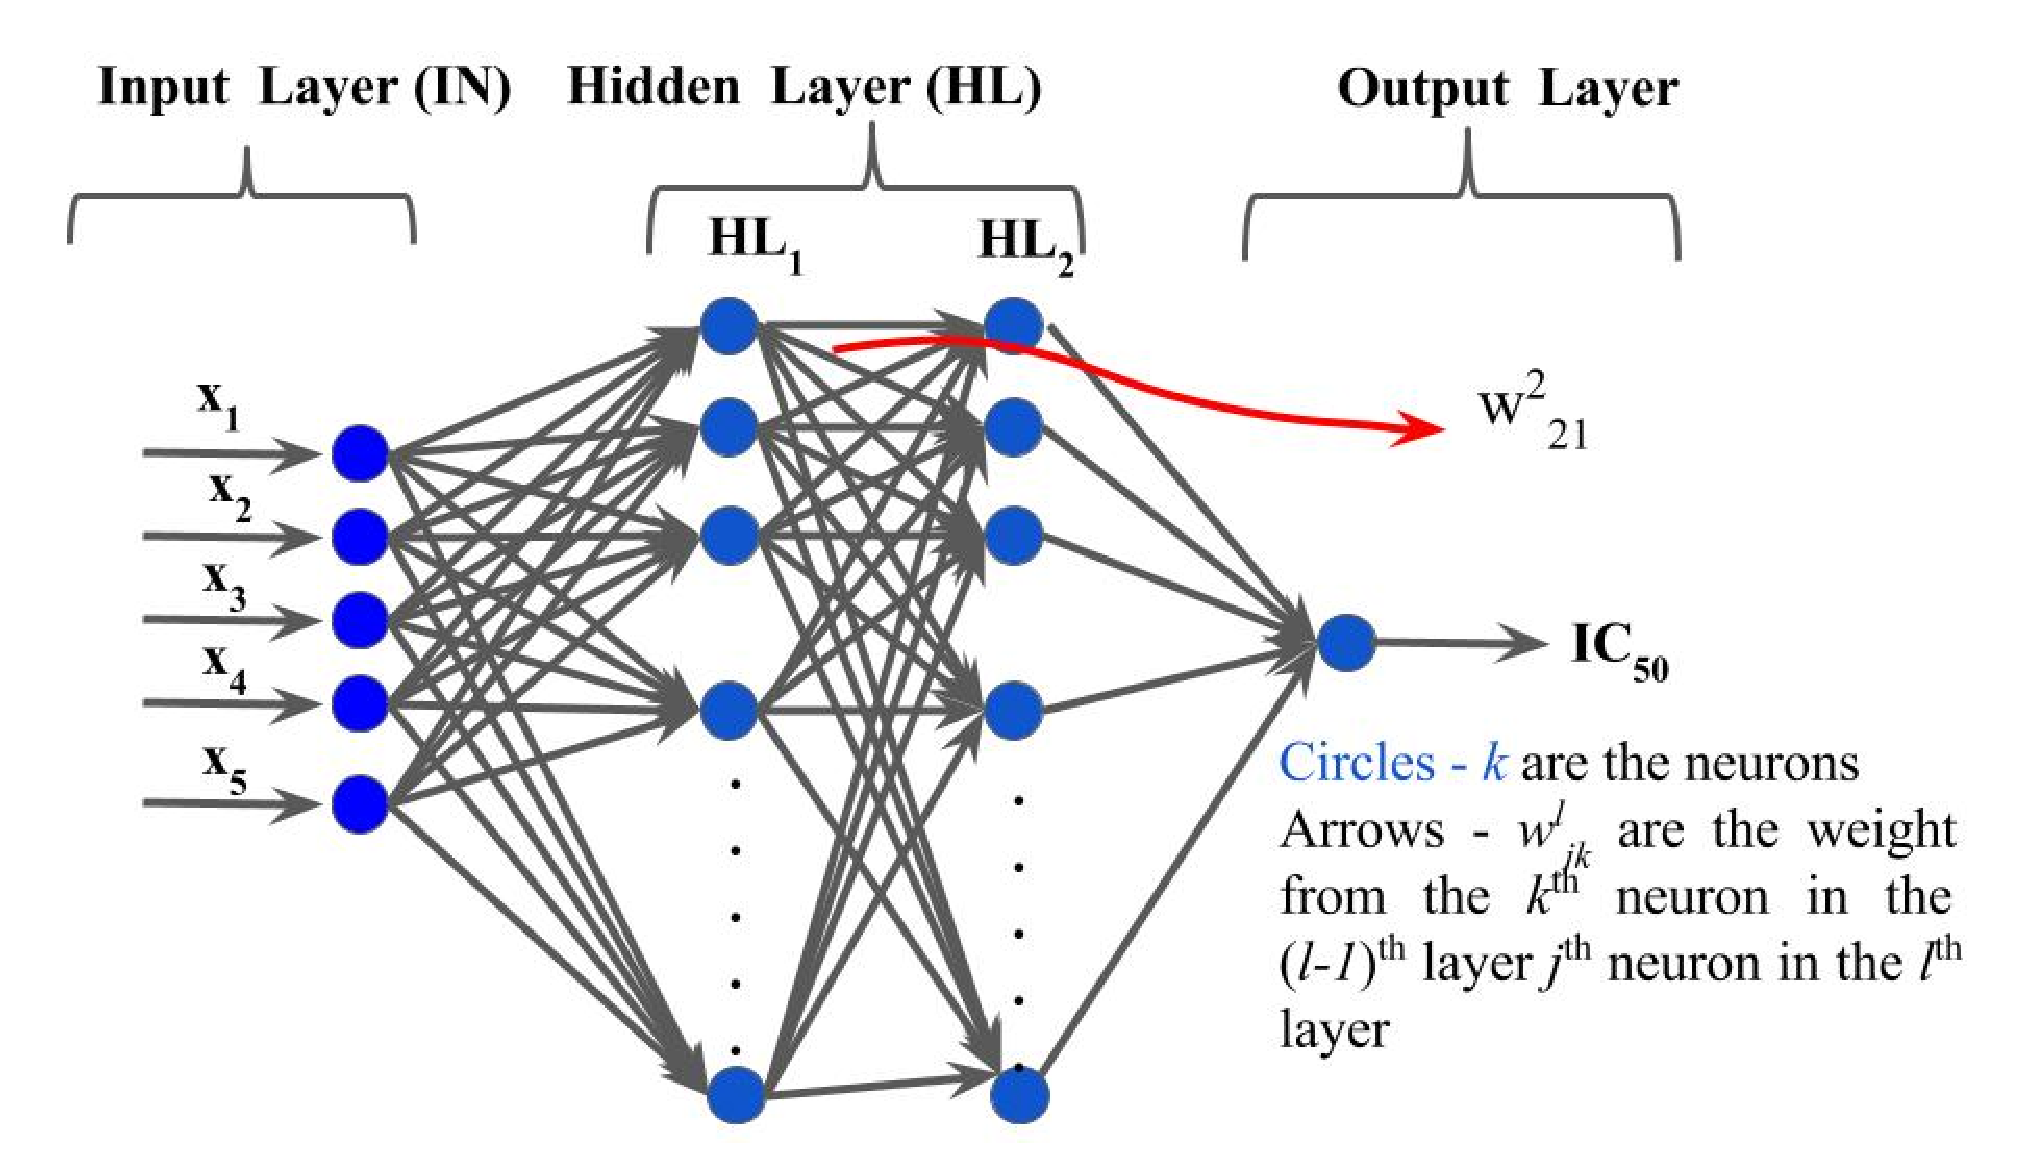
\includegraphics[clip=true,trim=0.1cm 0.1cm 0.1cm
                0cm,width=7cm]{ann.eps}
		\caption{The neural network model used in this project consists of four layers. The input layer consist of 5 principal components. Then two hidden layers and the final layer is the output layer which predicts the biological activity of the drug molecule. Here, $W$ represents the weights. The error $\delta$ is computed based on comparison between the biological activity predicted and the literature values $y$.
              Out of the 28 ligands considered in this study, 18 ligands are treated as training and the rest are
          treated as test data set. The 5 features of the drugs are classified as: (ATS Moreau-Broto 1 vdW radius, no. of rigid
      bonds, valence charge index 0, I\_edge\_adj\_deg\_mag and chi 3 path)}
\label{fig:model}
\end{figure}

\begin{table}[htb]
  \caption{Observed and the calculated {\it log}$IC_{50}$ values using ANN for the 28
inhibitors. The molecules shown in color are the test data set.}
\label{tab:table2}
\begin{tabular}{llll}
\hline\noalign{\smallskip}
S.No & Observed {\it log}$IC_{50}$ & Calculated {\it log}$IC_{50}$ & residuals  \\
\noalign{\smallskip}\hline\noalign{\smallskip}
1 & 0.477121 & 0.4908 & -0.01368\\
2 &  1.00000 & 1.0089 & -0.0089\\
3 &  1.04139 & 1.0491 & -0.00771\\
\textcolor{red}{4} & \textcolor{red}{1.07918} & \textcolor{red}{1.0908} &
\textcolor{red}{-0.01162}\\
5 & 1.14613 & 1.1529 & -0.00677\\
6 & 1.17609 & 1.1829 & -0.00681\\
\textcolor{red}{7} & \textcolor{red}{1.17609} & \textcolor{red}{1.1826} &
\textcolor{red}{-0.00651}\\
\textcolor{red}{8} & \textcolor{red}{1.17609} & \textcolor{red}{1.1787} &
\textcolor{red}{-0.00261}\\
9 & 1.47712 & 1.4796 & -0.00248\\
10 & 1.60206 & 1.6035 & -0.00144\\
\textcolor{red}{11} & \textcolor{red}{1.60206} & \textcolor{red}{1.6035} &
\textcolor{red}{-0.00144}\\
\textcolor{red}{12} & \textcolor{red}{1.65321} & \textcolor{red}{1.6512} &
\textcolor{red}{0.00201}\\
13 & 1.77815 & 1.7796 & -0.00145\\
\textcolor{red}{14} & \textcolor{red}{1.77815} & \textcolor{red}{1.7733} &
\textcolor{red}{0.00485}\\
\textcolor{red}{15} & \textcolor{red}{2.00000} & \textcolor{red}{1.9968} &
\textcolor{red}{0.0032}\\
16 & 2.30103 & 2.298 & 0.00303\\
17 & 2.30103 & 2.2962 & 0.00483\\
\textcolor{red}{18} & \textcolor{red}{2.30103} & \textcolor{red}{2.2989} &
\textcolor{red}{0.00213}\\
19 & 2.30103 & 2.2974 & 0.00363\\
20 & 2.30103 & 2.2983 & 0.00273\\
\textcolor{red}{21} & \textcolor{red}{2.39794} & \textcolor{red}{2.3928} &
\textcolor{red}{0.00514}\\
22 & 2.47712 & 2.4693 & 0.00782\\
\textcolor{red}{23} & \textcolor{red}{2.47712} &\textcolor{red}{2.4726} &
\textcolor{red}{0.00452}\\
24 & 2.477127 & 2.4738 & 0.00332\\
25 & 2.54407 & 2.541 & 0.00307 \\
26 & 2.60206 & 2.5977 & 0.00436\\
27 & 2.69897 & 2.6955 & 0.00347\\
28 & 3.00000 & 2.9883 & 0.0117\\
\noalign{\smallskip}\hline
\end{tabular}
\end{table}

\begin{table}[htb]
\caption{Statistical parameters of correlated data set using ANN method. Here
  $r^2$ is the correlation coefficient, $q^2$  is the cross validated
  correlation coefficient and MSE is the mean squared error.}
\label{tab:table3}
\begin{tabular}{lllll}
\hline\noalign{\smallskip}
S.No & $r^2$ & $q^2$ & MSE & No. of descriptors \\
\noalign{\smallskip}\hline\noalign{\smallskip}
1 &  0.7956 & 0.7955 & 0.0111 & 1\\
2 & 0.9543 & 0.9542 & 0.0036 & 2\\
3 & 0.9738 & 0.9735 & 0.0017 & 3\\
4 & 0.9868 & 0.9864 & 0.0008 & 4\\
5 & 0.9999 & 0.9999 & 0.0001 & 5\\
\noalign{\smallskip}\hline
\end{tabular}
\end{table}
\clearpage
\section{Conclusion}
New molecules can be now designed based on the 5 features (shown in table \ref{tab:table1}) and its respective biological activity can be known. A potential drug candidate should show less biological activity.
\bibliographystyle{spbasic}      % basic style, author-year citations
\bibliography{ref}  

\end{document}
